%!TEX root = ../ArticleCalib_main.tex
%!TEX root = ../sections/articleCalib_section4_SinglePixResponse

%%%%%%% FIGURE 1  : SINGLE PIX RESPONSE / HISTO CDF

\newgeometry{top=10mm}

\begin{figure}[]
\begin{center}
\captionsetup[subfigure]{position=top, labelfont=bf, textfont=normalfont, singlelinecheck=off, justification=raggedright }

\subfloat[]{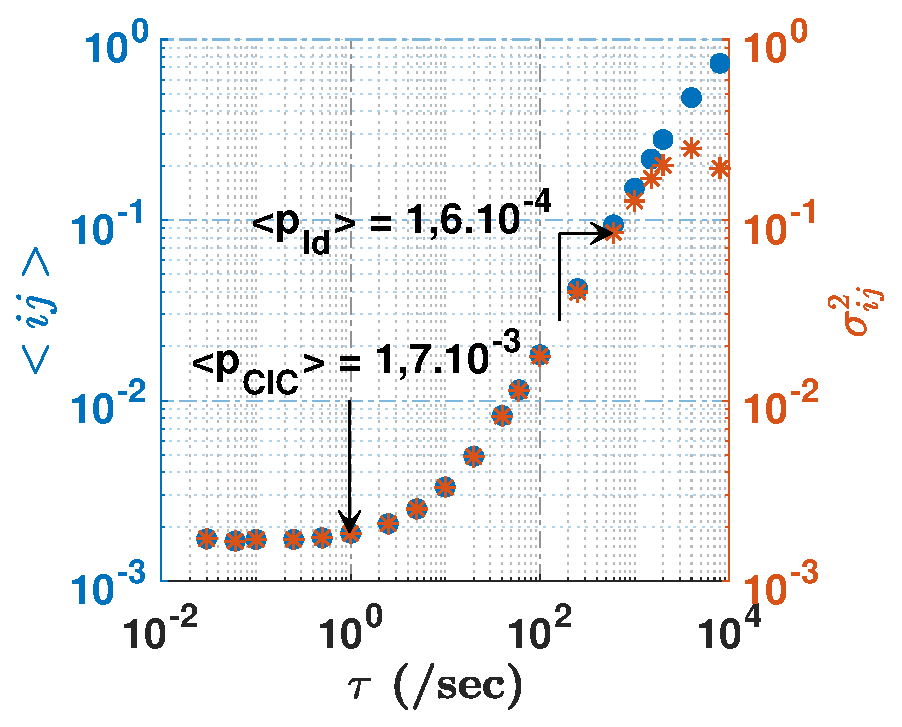
\includegraphics[width=0.40\linewidth]{fig1_caractSinglePixresponse/fig1A_meanvarIJ_Tau.eps}\label{fig:PixByPix:A}}  \\

\subfloat[]{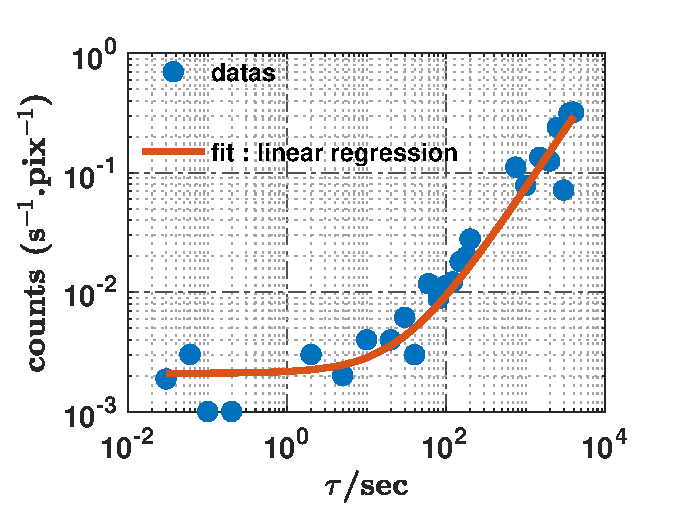
\includegraphics[width=0.40\linewidth]{fig1_caractSinglePixresponse/fig1B_fitmodel_MEF_170808_testLinFitWeighteddataPixIndex30010.eps}\label{fig:PixByPix:B}}\qquad
\subfloat[]{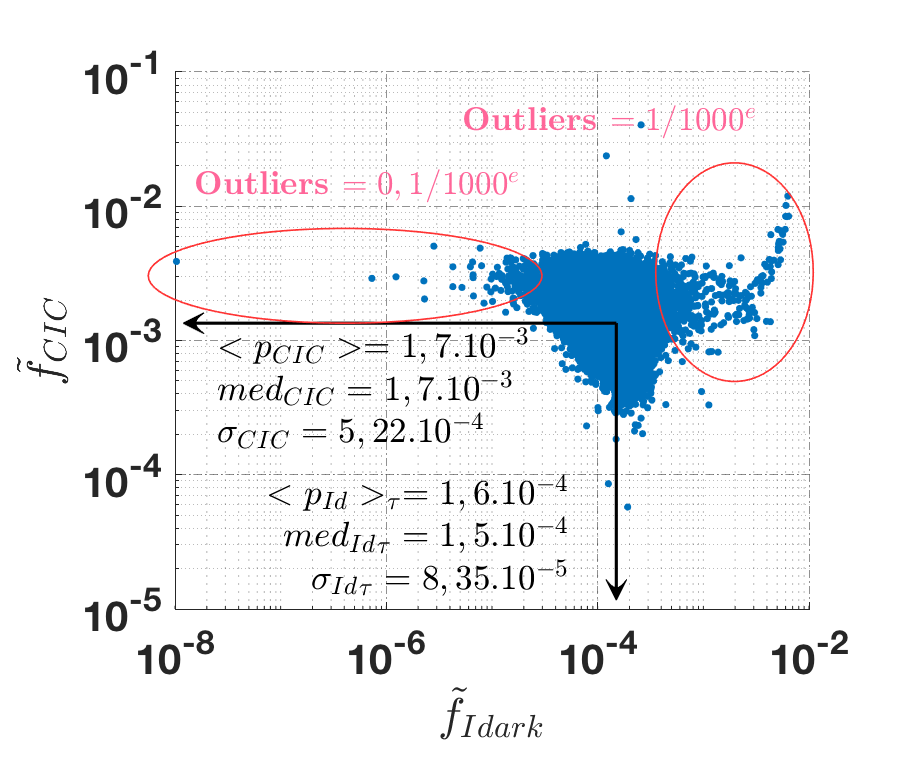
\includegraphics[width=0.4\linewidth]{fig1_caractSinglePixresponse/fig1C_PlotbiParam.eps}\label{fig:PixByPix:C}}  \\

\subfloat[]{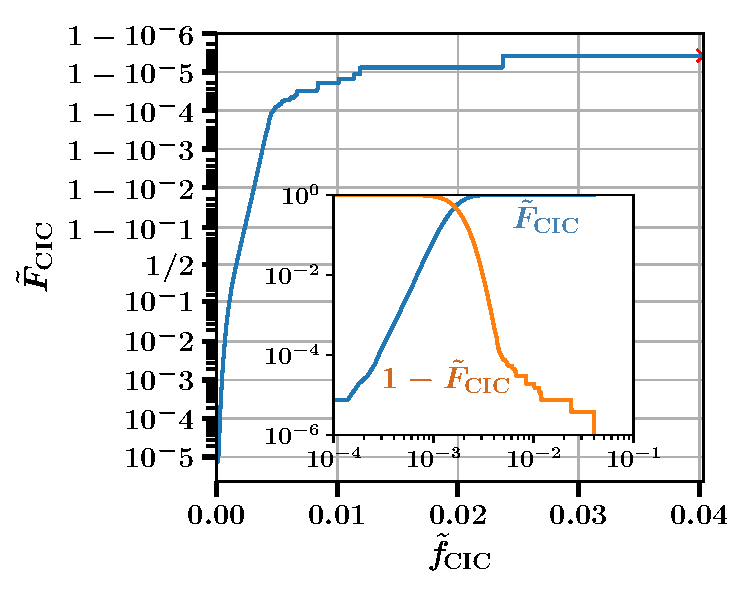
\includegraphics[width=0.40\linewidth]{fig1_caractSinglePixresponse/fig1D_E_CumSumCIC_Python.pdf}\label{fig:PixByPix:D}} \qquad
\subfloat[]{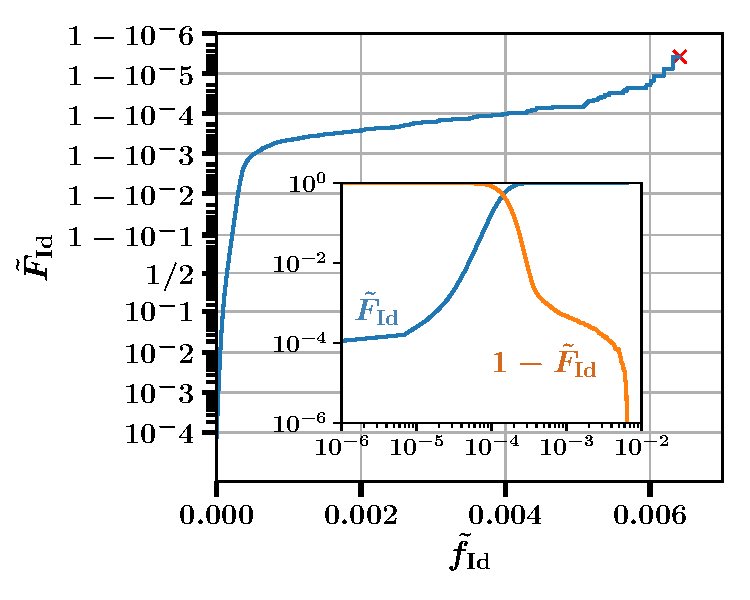
\includegraphics[width=0.40\linewidth]{fig1_caractSinglePixresponse/fig1D_E_CumSumId_Python.pdf}\label{fig:PixByPix:E}}. \\

\subfloat[]{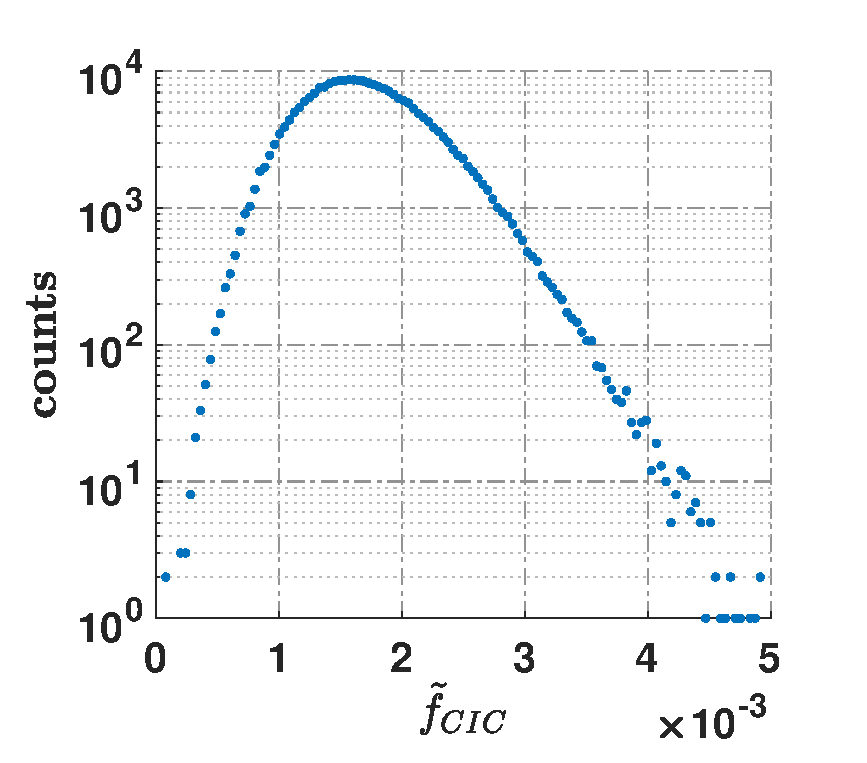
\includegraphics[width=0.35\linewidth]{fig1_caractSinglePixresponse/fig1F_G_HistoCIC.eps}\label{fig:PixByPix:F}} \qquad
\subfloat[]{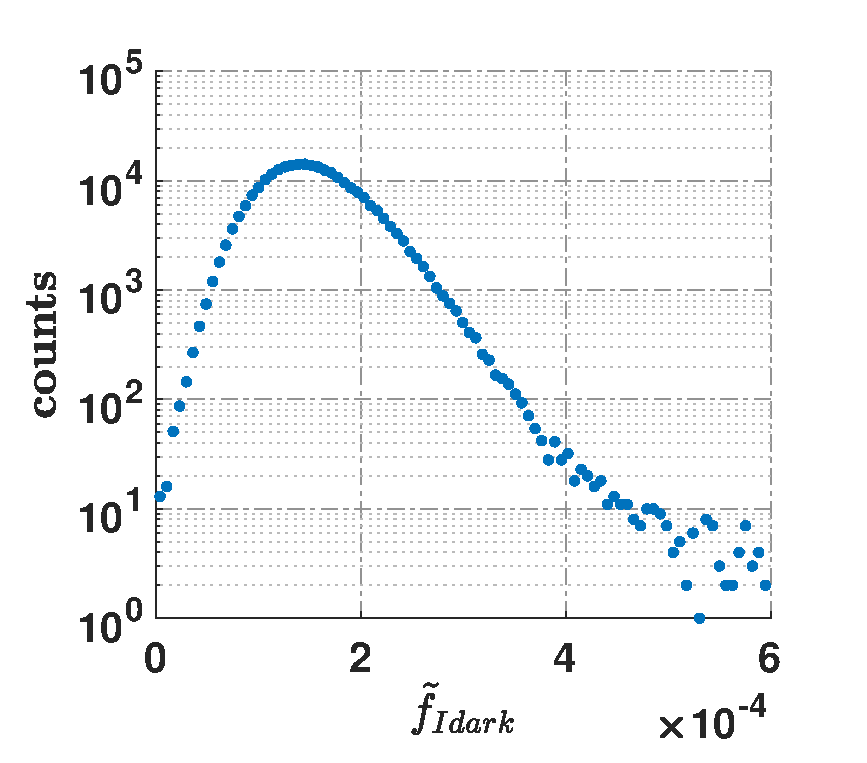
\includegraphics[width=0.35\linewidth]{fig1_caractSinglePixresponse/fig1F_G_HistoId.eps}\label{fig:PixByPix:G}} \\ 


\caption{{\bf Global detector response.} Evolution of the frequency of counts with the time of exposure  \subref{fig:PixByPix:A} .
{\bf single pixel : exemple of fit.} The individual pixel average noise response to an increased time of exposure $\tau$  was extracted and fitted out of saturation by weighted linear regression \subref{fig:PixByPix:B}. In those conditions the linear response is considered such as  <pixel$_{ij}$>$_K$$= CIC + Id * \tau$.
{\bf Caracterisation of single pixel response.} Single pixel response statistics \subref{fig:PixByPix:C}.  
Cumulative distribution (CDF) of the Clock Induced Charges (CIC) noise \subref{fig:PixByPix:D} and  the dark current (Id) \subref{fig:PixByPix:E} : Arctanh transform representation with insert in logarithmic scale  of the CDF and 1-CDF.
Histograms of the CIC \subref{fig:PixByPix:F} and the Id  \subref{fig:PixByPix:G}.}
\label{fig:PixByPix}
\end{center}
\end{figure}

\restoregeometry 
